\begin{frame}
    \frametitle{学科背景}
    \begin{figure}[H]
        \centering
        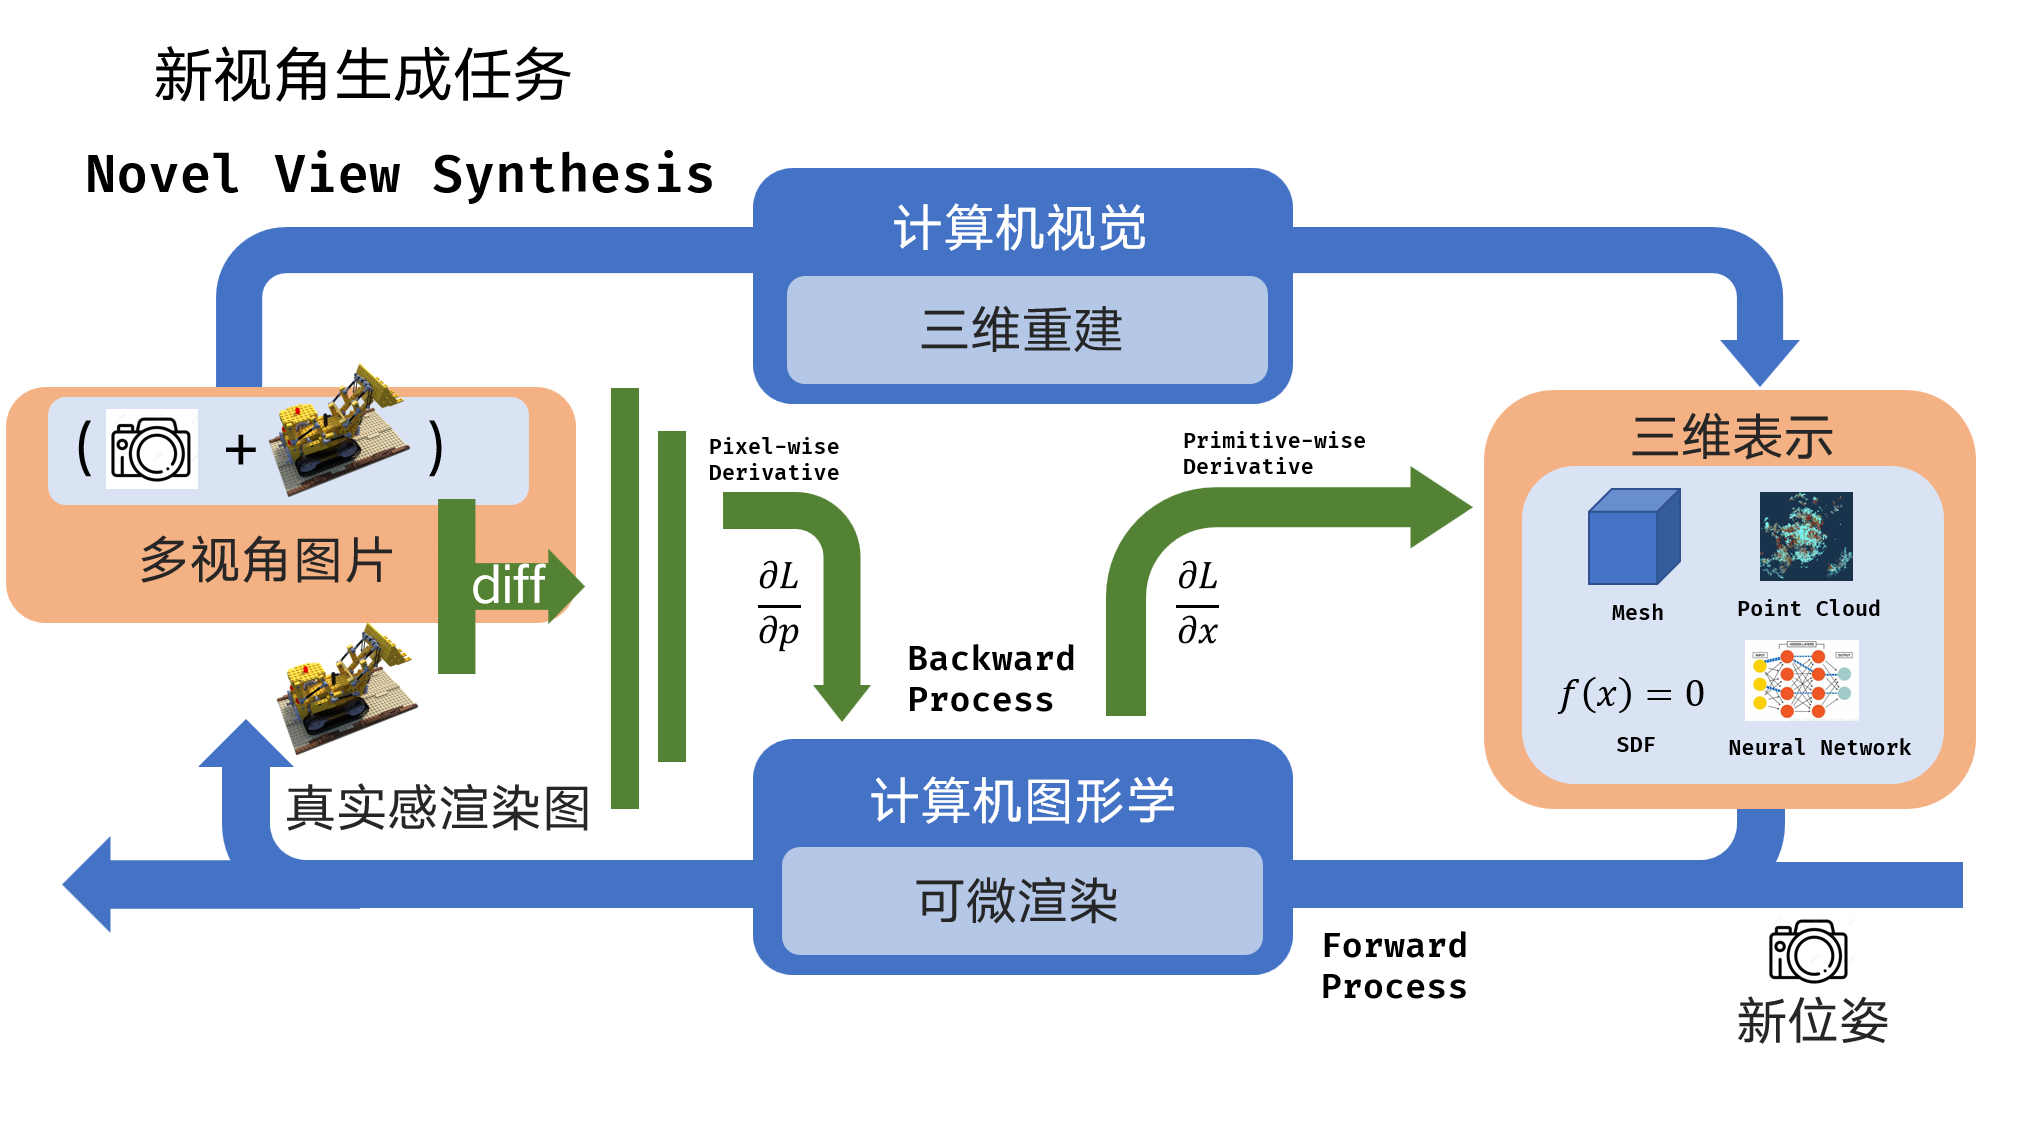
\includegraphics[width=1\linewidth,keepaspectratio]{fig_research_overview.png}
        \caption{学科背景和概述}
        \label{fig:research_overview}
    \end{figure}
\end{frame}

\begin{frame}
    \frametitle{计算机图形学}
    \begin{quote}
        传统意义上,计算机图形学是一门研究如何利用的三维表示和相机模型,
        模拟预测出真实感2D图形并绘制在屏幕上的学科
    \end{quote}
    \begin{figure}[H]
        \centering
        \includegraphics[width=1\linewidth,keepaspectratio]{fig_overview_graphics.png}
        \caption{计算机图形学}
        \label{fig:graphics_overview}
    \end{figure}
\end{frame}

\begin{frame}
    \frametitle{计算机图形学的应用}
    \begin{figure}[ht!]
        \centering
        \begin{subfigure}{0.3\textwidth}
            \centering
            \includegraphics[width=\textwidth]{fig_app_animations_graphics.png}
            \caption{动画}
        \end{subfigure}
        \begin{subfigure}{0.3\textwidth}
            \includegraphics[width=\textwidth]{fig_app_design_graphics.png}
            \caption{设计}
        \end{subfigure}
        \begin{subfigure}{0.3\textwidth}
            \centering
            \includegraphics[width=\textwidth]{fig_app_movie_graphics.png}
            \caption{电影}
        \end{subfigure}
        \begin{subfigure}{0.3\textwidth}
            \includegraphics[width=\textwidth]{fig_app_game_graphics.png}
            \caption{游戏}
        \end{subfigure}
        \begin{subfigure}{0.3\textwidth}
            \centering
            \includegraphics[width=\textwidth]{fig_app_gui_graphics.png}
            \caption{交互界面}
        \end{subfigure}
        \begin{subfigure}{0.3\textwidth}
            \includegraphics[width=\textwidth]{fig_app_visualization_graphics.png}
            \caption{可视化}
        \end{subfigure}
        \caption{计算机图形学的应用}
        \label{fig:app_computer_graphics}
    \end{figure}
\end{frame}

\begin{frame}
    \frametitle{光栅化}
    \begin{figure}[H]
        \centering
        \begin{subfigure}{0.68\textwidth}
            \centering
            \includegraphics[width=\textwidth]{fig_raster_projection.png}
            \caption{光栅化投影:\\ 按物体并行}
        \end{subfigure}
        \begin{subfigure}{0.3\textwidth}
            \includegraphics[width=\textwidth]{fig_raster_sample.png}
            \caption{光栅化采样:\\ 按像素并行}
        \end{subfigure}
    \end{figure}
\end{frame}

\begin{frame}
    \frametitle{光线追踪}
    \begin{figure}[ht!]
        \centering
        \begin{subfigure}{0.48\textwidth}
            \centering
            \includegraphics[width=\textwidth]{fig_ray_tracing_render.png}
            \caption{光线追踪过程示意}
        \end{subfigure}
        \begin{subfigure}{0.48\textwidth}
            \includegraphics[width=\textwidth]{fig_ray_tracing_result_render.png}
            \caption{光线追踪结果}
        \end{subfigure}
    \end{figure}
    \begin{quote}
        按屏幕像素进行并行
    \end{quote}
\end{frame}

